% ============================================================
%  يُترجَم بـ XeLaTeX  (في Overleaf: Menu → Compiler → XeLaTeX)
%  الخط: Amiri (متوفر في Overleaf، أو حمّله من github.com/aliftype/amiri)
% ============================================================
\documentclass[12pt,a4paper]{article}
\usepackage[a4paper,margin=1.7cm,top=2.3cm,bottom=2.9cm,headheight=15pt,footskip=1.5cm]{geometry}
\usepackage{amsmath,amssymb}
\usepackage{icomma}
\usepackage[english,bidi=default,layout=lists]{babel}
\babelprovide[import,main]{arabic}
\babelfont{rm}[Scale=1.08]{Amiri}
\babelfont{sf}[Scale=1.08]{Amiri}
\usepackage[most]{tcolorbox}
\usepackage{tikz}
\usetikzlibrary{arrows.meta,calc,shadings}
\usepackage{array}
\usepackage{colortbl}
\usepackage{fancyhdr}
\usepackage{titlesec}
\usepackage{enumitem}
\usepackage{collcell}
\usepackage{needspace}
\usepackage{etoolbox}
\newcolumntype{C}{>{\collectcell\ar}c<{\endcollectcell}}
\pretocmd{\section}{\Needspace{15\baselineskip}}{}{}
\pretocmd{\subsection}{\Needspace{11\baselineskip}}{}{}

\definecolor{cDef}{HTML}{1F4E9C}
\definecolor{cThm}{HTML}{B3261E}
\definecolor{cRem}{HTML}{2E7D32}
\definecolor{cEx}{HTML}{C76B00}
\definecolor{cMeth}{HTML}{6A1B9A}
\definecolor{cSol}{HTML}{00695C}
\definecolor{cSec}{HTML}{1F3A68}

\titleformat{\section}{\Large\bfseries\color{cSec}}{\thesection.}{0.6em}{}[{\color{cSec!60}\titlerule[1pt]}]
\titleformat{\subsection}{\large\bfseries\color{cThm!85!black}}{\thesubsection.}{0.5em}{}
\titlespacing*{\section}{0pt}{14pt}{8pt}
\titlespacing*{\subsection}{0pt}{10pt}{5pt}
\setlength{\parindent}{0pt}
\setlength{\parskip}{4pt}
\setlist{itemsep=2pt,topsep=3pt}

\newtcolorbox{arbox}[3][]{enhanced,
  colback=#2!5,colframe=#2!80!black,arc=2mm,boxrule=0.8pt,
  left=6pt,right=6pt,top=8pt,bottom=5pt,
  fonttitle=\bfseries,coltitle=white,
  title={\foreignlanguage{arabic}{#3}},
  attach boxed title to top right={xshift=-5mm,yshift=-3mm},
  boxed title style={colback=#2!80!black,arc=1.5mm,boxrule=0pt},
  before upper={\selectlanguage{arabic}},
  before skip=8pt,after skip=8pt,breakable,#1}
\newenvironment{BOX}[2]{\begin{otherlanguage}{english}\begin{arbox}{#1}{#2}}{\end{arbox}\end{otherlanguage}}
\newenvironment{tarif}[1][تعريف]{\begin{BOX}{cDef}{#1}}{\end{BOX}}
\newenvironment{khassia}[1][خاصية]{\begin{BOX}{cThm}{#1}}{\end{BOX}}
\newenvironment{molahada}[1][ملاحظة]{\begin{BOX}{cRem}{#1}}{\end{BOX}}
\newenvironment{mithal}[1][مثال]{\begin{BOX}{cEx}{#1}}{\end{BOX}}
\newenvironment{tariqa}[1][طريقة]{\begin{BOX}{cMeth}{#1}}{\end{BOX}}

\newcounter{exo}
\newenvironment{tamrin}[1]{\stepcounter{exo}\begin{BOX}{cSec}{التمرين \theexo: #1}}{\end{BOX}}
\newenvironment{hal}{\Needspace{12\baselineskip}\begin{otherlanguage}{english}\begin{arbox}[breakable]{cSol}{حل التمرين \theexo}}{\end{arbox}\end{otherlanguage}}

\newenvironment{LTR}{\begin{otherlanguage}{english}}{\end{otherlanguage}}
\newcommand{\ar}[1]{\foreignlanguage{arabic}{#1}}

\renewcommand{\dots}{\mathinner{\ldotp\ldotp\ldotp}}
\renewcommand{\ldots}{\mathinner{\ldotp\ldotp\ldotp}}
\renewcommand{\cdots}{\mathinner{\cdotp\cdotp\cdotp}}
\newcommand{\N}{\mathbb{N}}
\newcommand{\Z}{\mathbb{Z}}
\newcommand{\D}{\mathbb{D}}
\newcommand{\Q}{\mathbb{Q}}
\newcommand{\R}{\mathbb{R}}
\newcommand{\pgcd}{\operatorname{PGCD}}
\newcommand{\ppcm}{\operatorname{PPCM}}

% \NLseg{a}{b}{[}{]} ; \NLright{a}{[} ; \NLleft{b}{]}  (interval on a number line)
\newcommand{\NLseg}[4]{\begin{LTR}\begin{tikzpicture}[baseline=-0.6ex]
 \draw[-{Stealth[length=2mm]},gray!70](0,0)--(3.4,0);
 \draw[line width=2pt,cThm!80!black](0.7,0)--(2.7,0);
 \node[cThm!80!black,font=\LARGE] at (0.7,0){$#3$};
 \node[cThm!80!black,font=\LARGE] at (2.7,0){$#4$};
 \node[below=3pt,font=\footnotesize] at (0.7,0){$#1$};
 \node[below=3pt,font=\footnotesize] at (2.7,0){$#2$};
\end{tikzpicture}\end{LTR}}
\newcommand{\NLright}[2]{\begin{LTR}\begin{tikzpicture}[baseline=-0.6ex]
 \draw[-{Stealth[length=2mm]},gray!70](0,0)--(3.4,0);
 \draw[line width=2pt,cThm!80!black](1.3,0)--(3.3,0);
 \node[cThm!80!black,font=\LARGE] at (1.3,0){$#2$};
 \node[below=3pt,font=\footnotesize] at (1.3,0){$#1$};
\end{tikzpicture}\end{LTR}}
\newcommand{\NLleft}[2]{\begin{LTR}\begin{tikzpicture}[baseline=-0.6ex]
 \draw[-{Stealth[length=2mm]},gray!70](0,0)--(3.4,0);
 \draw[line width=2pt,cThm!80!black](0.05,0)--(2.1,0);
 \node[cThm!80!black,font=\LARGE] at (2.1,0){$#2$};
 \node[below=3pt,font=\footnotesize] at (2.1,0){$#1$};
\end{tikzpicture}\end{LTR}}

% ---------- social-media icons (pure TikZ) ----------
\definecolor{cFB}{HTML}{1877F2}
\definecolor{cTG}{HTML}{229ED9}
\definecolor{cIG1}{HTML}{FEDA75}
\definecolor{cIG2}{HTML}{D62976}
\definecolor{cIG3}{HTML}{4F5BD5}
\newcommand{\fbicon}{\begin{LTR}\begin{tikzpicture}[baseline=-0.75ex,x=1em,y=1em]
 \fill[cFB] (0,0) circle (0.55);
 \node[white,inner sep=0,font=\usefont{TU}{lmss}{bx}{n}\small] at (0.04,-0.02) {f};
\end{tikzpicture}\end{LTR}}
\newcommand{\igicon}{\begin{LTR}
\begin{tikzpicture}[baseline=-0.75ex,x=1em,y=1em]
 \shade[lower left=cIG1,lower right=cIG2,upper left=cIG2,upper right=cIG3,rounded corners=0.28em] (-0.55,-0.55) rectangle (0.55,0.55);
 \draw[white,line width=0.09em,rounded corners=0.18em] (-0.36,-0.36) rectangle (0.36,0.36);
 \draw[white,line width=0.09em] (0,0) circle (0.17);
 \fill[white] (0.22,0.22) circle (0.05);
\end{tikzpicture}\end{LTR}}
\newcommand{\tgicon}{\begin{LTR}
\begin{tikzpicture}[baseline=-0.75ex,x=1em,y=1em]
 \fill[cTG] (0,0) circle (0.55);
 \fill[white] (-0.33,0.0) -- (0.32,0.27) -- (0.2,-0.3) -- (0.0,-0.15) -- (-0.08,-0.28) -- (-0.08,-0.08) -- cycle;
 \fill[cTG!70!black] (-0.08,-0.08) -- (0.25,0.2) -- (0.0,-0.15) -- (-0.08,-0.28) -- cycle;
\end{tikzpicture}\end{LTR}}
% page number: black box, white two-digit number, at the right of the social row
\newcommand{\PageBox}{\begin{LTR}\tikz[baseline=(p.base)]\node[fill=black,text=white,inner sep=2.5pt,minimum width=1.6em,minimum height=1.3em,font=\usefont{TU}{lmss}{bx}{n}\small](p){\ifnum\value{page}<10 0\fi\arabic{page}};\end{LTR}}
% visual left-to-right order: Telegram | Instagram | Facebook | page box
\newcommand{\SocialRow}{\begin{otherlanguage}{english}%
 \ar{\textbf{الأستاذ سوايسية هشام للرياضيات}}\ \tgicon\hfill
 \textbf{prof\_hicham\_math}\ \igicon\hfill
 \ar{\textbf{الأستاذ سوايسية هشام للرياضيات}}\ \fbicon\hspace{2.2em}\PageBox\end{otherlanguage}}

\pagestyle{fancy}
\fancyhf{}
\renewcommand{\headrulewidth}{0.6pt}
\renewcommand{\footrulewidth}{0.4pt}
% \SetHeader{right head: document title}{left head: level -- stream}
\newcommand{\SetHeader}[2]{%
 \fancyhead[C]{\parbox{\textwidth}{\ar{#1\hfill #2}}}%
 \fancyfoot[C]{\parbox{\textwidth}{\small\SocialRow}}}
\usepackage{tkz-tab}
\usepackage{multicol}
% variation / sign table (LTR)
\newenvironment{TAB}{\par\begin{center}\begin{LTR}\begin{tikzpicture}[scale=0.95,every node/.style={font=\small}]}{\end{tikzpicture}\end{LTR}\end{center}}
% grid + axes, clipped: \begin{GR}{xmin}{xmax}{ymin}{ymax}{unit cm}
\newenvironment{GR}[5]{\par\begin{center}\begin{LTR}\begin{tikzpicture}[x=#5cm,y=#5cm,font=\footnotesize]
 \draw[gray!25,very thin] (#1,#3) grid (#2,#4);
 \draw[-{Stealth[length=2mm]}] (#1,0)--(#2+0.3,0) node[below left]{$x$};
 \draw[-{Stealth[length=2mm]}] (0,#3)--(0,#4+0.3) node[below left]{$y$};
 \node[below left] at (0,0){$O$};
 \begin{scope}\clip (#1,#3) rectangle (#2,#4);}
{\end{scope}\end{tikzpicture}\end{LTR}\end{center}}
\newcommand{\Ticks}[2]{\foreach \t in {#1} \node[below,font=\scriptsize] at (\t,0){$\t$}; \foreach \t in {#2} \node[left,font=\scriptsize] at (0,\t){$\t$};}
\newcommand{\bx}[1]{\ensuremath{\colorbox{cDef!12}{$\displaystyle #1$}}}
\newcommand{\TwoCol}[4]{\par\begin{LTR}\noindent\begin{minipage}[t]{#1\textwidth}\selectlanguage{arabic}#2\end{minipage}\hfill\begin{minipage}[t]{#3\textwidth}\selectlanguage{arabic}#4\end{minipage}\end{LTR}\par}
\newcommand{\RL}[4]{\TwoCol{#3}{#4}{#1}{#2}}  % \RL{w1}{right content}{w2}{left content}
\newcommand{\ok}{$\textcolor{cRem}{\checkmark}$}
\newcommand{\limn}{\displaystyle\lim_{n\to+\infty}}
% sub-questions, each on its own line
\newenvironment{sq}{\begin{itemize}[leftmargin=2.4em,itemsep=3pt]}{\end{itemize}}
\newcommand{\qa}{\item[(أ)]}\newcommand{\qb}{\item[(ب)]}\newcommand{\qc}{\item[(جـ)]}\newcommand{\qd}{\item[(د)]}\newcommand{\qe}{\item[(هـ)]}
\newcommand{\pa}{\par\smallskip\textbf{(أ)} }\newcommand{\pb}{\par\smallskip\textbf{(ب)} }\newcommand{\pc}{\par\smallskip\textbf{(جـ)} }\newcommand{\pd}{\par\smallskip\textbf{(د)} }\newcommand{\pe}{\par\smallskip\textbf{(هـ)} }
\newcommand{\QQ}[1]{\par\smallskip\textbf{#1.} }
\newenvironment{tmr}{\stepcounter{exo}\begin{BOX}{cSec}{تمرين محلول \theexo}}{\end{BOX}}
\newcommand{\ABC}[3]{\\[2pt]\begin{tabular}{p{0.28\textwidth}p{0.28\textwidth}p{0.28\textwidth}}(جـ) \ #3 & (ب) \ #2 & (أ) \ #1\end{tabular}}
\pretocmd{\section}{\Needspace{24\baselineskip}}{}{}
\newtcbox{\bxtbox}{on line,colback=cDef!12,colframe=cDef!12,boxrule=0pt,arc=1pt,boxsep=0pt,left=2pt,right=2pt,top=1pt,bottom=1pt}
\newcommand{\bxt}[1]{\foreignlanguage{english}{\bxtbox{\ar{#1}}}}
\usepackage{longtable}
\setlength{\LTpre}{4pt}\setlength{\LTpost}{0pt}
\newcommand{\Phase}[1]{\textbf{#1}}
\newcommand{\Fld}[2]{\textbf{#1:}\ #2}
% رأس المذكرة على نمط النموذج: إطار بعنوان «مذكرة رقم»، معلومات الحصة، ثم إطار الكفاءات
\newcommand{\ModhHead}[9]{%
\begin{LTR}
\begin{tcolorbox}[enhanced,colback=white,colframe=cThm!85!black,arc=4mm,boxrule=1pt,top=14pt,bottom=6pt,left=8pt,right=8pt,
 overlay={\node[fill=cThm!85!black,text=white,rounded corners=3mm,inner xsep=14pt,inner ysep=4pt,font=\large\bfseries] at ([yshift=0pt]frame.north){\ar{مذكرة رقم #1}};},
 before upper={\selectlanguage{arabic}}]
\begin{tabular}{@{}p{0.4\linewidth}p{0.55\linewidth}@{}}
\Fld{المستوى}{#2} & \Fld{الثانوية}{\dotfill}\\[3pt]
\Fld{المادة}{رياضيات} & \Fld{ميدان التعلم}{#3}\\[3pt]
\Fld{المدة}{#5} & \Fld{الوحدة التعلمية}{#4}\\[3pt]
\Fld{الأستاذ}{\dotfill} & \Fld{المحتوى المعرفي}{#6}\\
\end{tabular}
\end{tcolorbox}
\begin{tcolorbox}[enhanced,colback=white,colframe=cThm!85!black,arc=3mm,boxrule=0.8pt,sidebyside,sidebyside align=top,lefthand ratio=0.5,
 segmentation style={dashed,cThm!60},before upper={\selectlanguage{arabic}},before lower={\selectlanguage{arabic}}]
\textbf{الكفاءات المستهدفة:}\par #8
\tcblower
\textbf{الكفاءات القبلية:}\par #7
\end{tcolorbox}
\end{LTR}
\par\smallskip\textbf{الوسائل:} #9\par\smallskip}
\newenvironment{Sayr}{%
\begin{LTR}\renewcommand{\arraystretch}{1.25}
\begin{longtable}{|p{0.17\textwidth}|>{\centering\arraybackslash}p{0.06\textwidth}|p{0.53\textwidth}|>{\centering\arraybackslash}p{0.12\textwidth}|}
\hline\rowcolor{cThm!12}\ar{\textbf{توجيهات وتعاليق}} & \ar{\textbf{المدة}} & \ar{\textbf{سير الحصة}} & \ar{\textbf{مراحل الحصة}}\\\hline\endhead
\hline\endfoot}{\end{longtable}\end{LTR}}
% سطر في الجدول: \Row{مرحلة}{سير}{مدة}{توجيهات}
\newcommand{\Row}[4]{\ar{\small #4} & \ar{#3} & \ar{#2} & \cellcolor{cThm!8}\ar{\Phase{#1}}\\\hline}

\newcommand{\Lab}[2]{\foreignlanguage{english}{\tcbox[on line,colback=#1,colframe=#1,boxrule=0pt,arc=2pt,boxsep=1pt,left=5pt,right=5pt,top=1pt,bottom=1pt]{\ar{\textcolor{white}{\textbf{#2}}}}}}
\newcommand{\Num}[1]{\foreignlanguage{english}{\tikz[baseline=(c.base)]\node[fill=cDef,text=white,inner sep=2pt,font=\footnotesize\bfseries](c){#1};}}
\newcommand{\ck}{\ensuremath{{\color{cRem}\checkmark}}}
\newenvironment{Kad}[1]{\par\smallskip\Lab{#1}}{\par}
\SetHeader{\small\bfseries\color{cSec}مذكرات محور: المرجح في المستوي}{\small\color{cSec}السنة الثانية ثانوي -- علوم تجريبية}
\begin{document}
\begin{LTR}
\begin{tcolorbox}[enhanced,colback=cThm!85!black,colframe=cThm!85!black,arc=3mm,halign=center,boxrule=0pt,top=12pt,bottom=12pt,before upper={\selectlanguage{arabic}}]
{\color{white}\fontsize{26}{32}\selectfont\bfseries مذكرات محور: المرجح في المستوي}\\[8pt]
{\color{white}\large السنة الثانية ثانوي -- علوم تجريبية (صالحة لشعبتي رياضيات وتقني رياضي)}\\[4pt]
{\color{white}\large 6 مذكرات (12 ساعة) -- السنة الدراسية 2026-2027}
\end{tcolorbox}
\end{LTR}
\begin{BOX}{cThm}{يتضمن هذا العمل}
\begin{enumerate}[label=\textbf{مذكرة \arabic{enumi}:},leftmargin=6em,start=25]
\item مرجح نقطتين.
\item مرجح ثلاث نقط.
\item خاصية التجميع (المرجح الجزئي).
\item إحداثيا المرجح.
\item استقامية نقط وتلاقي مستقيمات.
\item مجموعات نقط: دراسة ، تعيين ، إنشاء.
\end{enumerate}
مراجع النشاطات والتمارين: الكتاب المدرسي للسنة الثانية ثانوي (باب المرجح).
\end{BOX}
\newpage
\ModhHead{25}{2 ع ت}{هندسة}{المرجح في المستوي}{02 سا}{مرجح نقطتين}%
{\begin{itemize}\item الأشعة: علاقة شال ، ضرب شعاع في عدد (1 ج م).\end{itemize}}%
{\begin{itemize}\item تعريف مرجح نقطتين وإنشاؤه.\item استعمال خواص مرجح نقطتين.\end{itemize}}%
{المنهاج ، الكتاب المدرسي ، مراجع ، أدوات الهندسة.}
\begin{Sayr}
\Row{مرحلة الانطلاق}{%
\textbf{التهيئة النفسية:} كيف يتوازن طفلان مختلفا الكتلة على أرجوحة؟ أين نضع المحور؟}{10 د}{وضعية فيزيائية.}
\Row{التشخيص والاكتشاف}{%
\Lab{cEx}{مناقشة نشاط 01 (أنشطة باب المرجح)}\par\ck\ قانون أرخميدس: التوازن يتحقق إذا كان $m_1\times GA=m_2\times GB$.\par
\ck\ شعاعياً: $m_1\overrightarrow{GA}+m_2\overrightarrow{GB}=\vec0$ ؛ النقطة $G$ نقطة توازن $A$ و $B$ المرفقتين بالكتلتين.\par
}{35 د}{نشاط الكتاب.}
\Row{بناء المعارف}{%
\Lab{cDef}{تعريف}\ $\alpha+\beta\neq0$: توجد نقطة وحيدة $G$ حيث $\alpha\overrightarrow{GA}+\beta\overrightarrow{GB}=\vec0$ ، نسميها \textbf{مرجح} الجملة $\{(A;\alpha),(B;\beta)\}$.\par\Lab{cThm}{الإنشاء}\ $\overrightarrow{AG}=\dfrac\beta{\alpha+\beta}\overrightarrow{AB}$ ، و $G\in(AB)$.\par}{50 د}{الإنشاء بالمسطرة.}
\Row{}{%
\Lab{cEx}{مثال}\ مرجح $\{(A;2),(B;1)\}$: $\overrightarrow{AG}=\frac13\overrightarrow{AB}$.\par\smallskip\begin{LTR}\centering 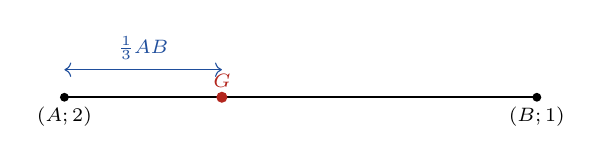
\begin{tikzpicture}[x=1cm,font=\scriptsize]
\draw[thick] (0,0)--(6,0);
\foreach \x/\n/\w in {0/A/2,6/B/1} {\fill (\x,0) circle (1.6pt); \node[below] at (\x,0){$(\n;\w)$};}
\fill[cThm] (2,0) circle (2pt) node[above]{$G$};
\draw[<->,cDef] (0,0.35)--(2,0.35) node[midway,above]{$\frac13AB$};
\end{tikzpicture}\end{LTR}\par \Lab{cThm}{خواص}\par\ck\ لا يتغير المرجح إذا ضربنا المعاملين في نفس العدد غير المعدوم.\par
\ck\ مرجح $\{(A;1),(B;1)\}$ هو منتصف $[AB]$.\par
\ck\ من أجل كل نقطة $M$: $\alpha\overrightarrow{MA}+\beta\overrightarrow{MB}=(\alpha+\beta)\overrightarrow{MG}$.\par
}{}{}
\Row{}{%
\Lab{cThm!80!black}{حذار}\ إذا كان $\alpha+\beta=0$ فلا يوجد مرجح.}{}{}
\Row{التقويم}{%
\Lab{cEx}{تطبيق}\par أنشئ $G$ مرجح $\{(A;3),(B;-1)\}$ و $H$ مرجح $\{(A;1),(B;3)\}$.\par\textbf{الحل:} $\overrightarrow{AG}=\dfrac{-1}{2}\overrightarrow{AB}$ ($G$ خارج $[AB]$ من جهة $A$) ؛ $\overrightarrow{AH}=\dfrac34\overrightarrow{AB}$.\par\textbf{واجب منزلي:} تمارين 18 إلى 28 من باب المرجح.\par\smallskip\textbf{ملاحظات حول سير الحصة:} \dotfill}{25 د}{تقويم فردي.}
\end{Sayr}
\newpage
\ModhHead{26}{2 ع ت}{هندسة}{المرجح في المستوي}{02 سا}{مرجح ثلاث نقط}%
{\begin{itemize}\item مرجح نقطتين.\end{itemize}}%
{\begin{itemize}\item تعريف مرجح ثلاث نقط وإنشاؤه.\end{itemize}}%
{المنهاج ، الكتاب المدرسي ، مراجع ، أدوات الهندسة.}
\begin{Sayr}
\Row{مرحلة الانطلاق}{%
\textbf{التهيئة النفسية:} كيف نوازن صفيحة مثلثة الشكل علقنا في رؤوسها كتلاً؟}{10 د}{وضعية فيزيائية.}
\Row{التشخيص والاكتشاف}{%
\Lab{cEx}{مناقشة نشاط 02 (أنشطة باب المرجح)}\par\ck\ مثلث $ABC$ ونقط معرفة بعلاقات شعاعية: إنشاؤها ، ثم إثبات استقامية نقط بعلاقة شال.\par
}{35 د}{عمل ثنائي.}
\Row{بناء المعارف}{%
\Lab{cDef}{تعريف}\ $\alpha+\beta+\gamma\neq0$: النقطة الوحيدة $G$ حيث $\alpha\overrightarrow{GA}+\beta\overrightarrow{GB}+\gamma\overrightarrow{GC}=\vec0$ هي مرجح $\{(A;\alpha),(B;\beta),(C;\gamma)\}$.\par\Lab{cThm}{خاصية}\ من أجل كل نقطة $M$: $\alpha\overrightarrow{MA}+\beta\overrightarrow{MB}+\gamma\overrightarrow{MC}=(\alpha+\beta+\gamma)\overrightarrow{MG}$ ؛ وبأخذ $M=A$: $\overrightarrow{AG}=\dfrac{\beta\overrightarrow{AB}+\gamma\overrightarrow{AC}}{\alpha+\beta+\gamma}$.\par}{50 د}{نرسم الأشعة بالألوان.}
\Row{}{%
\Lab{cEx}{مثال}\ $G$ مرجح $\{(A;1),(B;1),(C;1)\}$: $\overrightarrow{AG}=\frac13(\overrightarrow{AB}+\overrightarrow{AC})$ ، و $G$ مركز ثقل المثلث.\par\Lab{cDef}{مركز المسافات المتساوية}\ مرجح نقط معاملاتها متساوية.\par}{}{}
\Row{}{%
\Lab{cThm!80!black}{حذار}\ نتحقق دائماً أن مجموع المعاملات غير معدوم.}{}{}
\Row{التقويم}{%
\Lab{cEx}{تطبيق}\par أنشئ $G$ مرجح $\{(A;2),(B;1),(C;1)\}$.\par\textbf{الحل:} $\overrightarrow{AG}=\dfrac{\overrightarrow{AB}+\overrightarrow{AC}}4$ ؛ إذا كانت $I$ منتصف $[BC]$: $\overrightarrow{AB}+\overrightarrow{AC}=2\overrightarrow{AI}$ ، إذن $\overrightarrow{AG}=\frac12\overrightarrow{AI}$.\par\textbf{واجب منزلي:} تمارين 38 إلى 44 من باب المرجح.\par\smallskip\textbf{ملاحظات حول سير الحصة:} \dotfill}{25 د}{تقويم فردي.}
\end{Sayr}
\newpage
\ModhHead{27}{2 ع ت}{هندسة}{المرجح في المستوي}{02 سا}{خاصية التجميع (المرجح الجزئي)}%
{\begin{itemize}\item مرجح نقطتين وثلاث نقط.\end{itemize}}%
{\begin{itemize}\item استعمال خاصية التجميع لإنشاء مرجح.\end{itemize}}%
{المنهاج ، الكتاب المدرسي ، مراجع ، أدوات الهندسة.}
\begin{Sayr}
\Row{مرحلة الانطلاق}{%
\textbf{التهيئة النفسية:} معدلك الفصلي: هل يمكن حسابه انطلاقاً من معدل المواد الأدبية ومعدل المواد العلمية؟}{10 د}{وضعية المعدل.}
\Row{التشخيص والاكتشاف}{%
\Lab{cEx}{مناقشة نشاط 04 (أنشطة باب المرجح)}\par\ck\ معدل كل مجموعة مواد مع مجموع معاملاتها ، ثم المعدل العام بهذين المعدلين: نجد نفس النتيجة.\par
\ck\ هذه هي فكرة \textbf{التجميع}.\par
}{35 د}{حساب بالأرقام ثم تعميم.}
\Row{بناء المعارف}{%
\Lab{cThm}{خاصية التجميع}\ إذا كانت $H$ مرجح $\{(A;\alpha),(B;\beta)\}$ مع $\alpha+\beta\neq0$ ، فإن مرجح $\{(A;\alpha),(B;\beta),(C;\gamma)\}$ هو مرجح $\{(H;\alpha+\beta),(C;\gamma)\}$.\par\Lab{cEx}{مثال}\ $G$ مرجح $\{(A;1),(B;1),(C;2)\}$ ، $I$ منتصف $[AB]$: $G$ مرجح $\{(I;2),(C;2)\}$ ، أي منتصف $[IC]$.\par\smallskip\begin{LTR}\centering 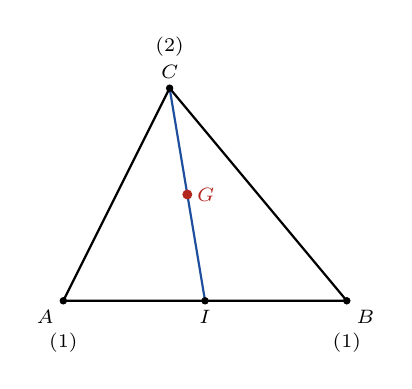
\begin{tikzpicture}[scale=0.9,font=\scriptsize]
\coordinate (A) at (0,0); \coordinate (B) at (4,0); \coordinate (C) at (1.5,3);
\coordinate (I) at (2,0); \coordinate (G) at (1.75,1.5);
\draw[thick] (A)--(B)--(C)--cycle; \draw[cDef,thick] (I)--(C);
\foreach \p/\pos in {A/below left,B/below right,C/above,I/below} {\fill (\p) circle (1.5pt) node[\pos]{$\p$};}
\fill[cThm] (G) circle (2pt) node[right]{$G$};
\node[below=8pt] at (A){$(1)$}; \node[below=8pt] at (B){$(1)$}; \node[above=8pt] at (C){$(2)$};
\end{tikzpicture}\end{LTR}\par }{50 د}{نرسم المرجح الجزئي بلون مختلف.}
\Row{}{%
\Lab{cRem}{ملاحظات}\ نجمع النقط التي يسهل إنشاء مرجحها (معاملات متساوية غالباً).\par\Lab{cThm!80!black}{حذار}\ لا نجمع نقطتين مجموع معامليهما معدوم.}{}{}
\Row{التقويم}{%
\Lab{cEx}{تطبيق}\par بيّن أن مركز ثقل مثلث يقع على كل متوسط وعلى ثلثيه من الرأس.\par\textbf{الحل:} $G$ مرجح $\{(A;1),(B;1),(C;1)\}$ ؛ $I$ منتصف $[BC]$: $G$ مرجح $\{(A;1),(I;2)\}$ ، إذن $\overrightarrow{AG}=\frac23\overrightarrow{AI}$.\par\textbf{واجب منزلي:} تمارين من باب المرجح.\par\smallskip\textbf{ملاحظات حول سير الحصة:} \dotfill}{25 د}{تقويم فردي.}
\end{Sayr}
\newpage
\ModhHead{28}{2 ع ت}{هندسة}{المرجح في المستوي}{02 سا}{إحداثيا المرجح}%
{\begin{itemize}\item المعلم ، إحداثيات شعاع (1 ج م) ، المرجح.\end{itemize}}%
{\begin{itemize}\item حساب إحداثيي مرجح في معلم.\end{itemize}}%
{المنهاج ، الكتاب المدرسي ، مراجع ، أدوات الهندسة.}
\begin{Sayr}
\Row{مرحلة الانطلاق}{%
\textbf{التهيئة النفسية:} ما إحداثيا منتصف القطعة $[AB]$ حيث $A(2;3)$ و $B(4;-1)$ ؟}{10 د}{تذكير.}
\Row{التشخيص والاكتشاف}{%
\Lab{cEx}{وضعية مقترحة}\ $G$ مرجح $\{(A;1),(B;2)\}$ مع $A(2;3)$ و $B(-1;0)$.\par\ck\ $\overrightarrow{AG}=\frac23\overrightarrow{AB}$: $x_G-2=\frac23(-3)$ ، $y_G-3=\frac23(-3)$ ، إذن $G(0;1)$.\par
\ck\ نلاحظ: $x_G=\dfrac{1\times2+2\times(-1)}3=0$ و $y_G=\dfrac{1\times3+2\times0}3=1$.\par
}{35 د}{الطريقتان: الشعاعية والدستور.}
\Row{بناء المعارف}{%
\Lab{cThm}{خاصية}\ $G$ مرجح $\{(A;\alpha),(B;\beta),(C;\gamma)\}$:\par\ck\ $x_G=\dfrac{\alpha x_A+\beta x_B+\gamma x_C}{\alpha+\beta+\gamma}$ ، $y_G=\dfrac{\alpha y_A+\beta y_B+\gamma y_C}{\alpha+\beta+\gamma}$.\par
\Lab{cEx}{مثال}\ $A(1;2)$ ، $B(4;-1)$ ، $C(-2;5)$ ، المعاملات $1$ ، $2$ ، $3$: $x_G=\dfrac{1+8-6}6=\dfrac12$ ، $y_G=\dfrac{2-2+15}6=\dfrac52$.\par}{50 د}{نتحقق بالرسم في المعلم.}
\Row{}{%
\Lab{cRem}{ملاحظات}\ الإحداثيان «متوسطان مرجحان» للإحداثيات ، كالمعدل الفصلي.\par\Lab{cThm!80!black}{حذار}\ نقسم على مجموع المعاملات لا على عدد النقط.}{}{}
\Row{التقويم}{%
\Lab{cEx}{تطبيق}\par $A(0;1)$ و $B(3;1)$. عيّن عددين $\alpha$ و $\beta$ حتى تكون $G(2;1)$ مرجح $\{(A;\alpha),(B;\beta)\}$.\par\textbf{الحل:} $\overrightarrow{AG}=\frac23\overrightarrow{AB}$ ، إذن $\dfrac\beta{\alpha+\beta}=\dfrac23$: مثلاً $\alpha=1$ ، $\beta=2$.\par\textbf{واجب منزلي:} تمارين 89 إلى 96 من باب المرجح.\par\smallskip\textbf{ملاحظات حول سير الحصة:} \dotfill}{25 د}{تقويم فردي.}
\end{Sayr}
\newpage
\ModhHead{29}{2 ع ت}{هندسة}{المرجح في المستوي}{02 سا}{استقامية نقط وتلاقي مستقيمات}%
{\begin{itemize}\item المرجح ، خاصية التجميع.\end{itemize}}%
{\begin{itemize}\item استعمال المرجح لإثبات استقامية نقط وتلاقي مستقيمات.\end{itemize}}%
{المنهاج ، الكتاب المدرسي ، مراجع ، أدوات الهندسة.}
\begin{Sayr}
\Row{مرحلة الانطلاق}{%
\textbf{التهيئة النفسية:} كيف نثبت أن ثلاث نقط على استقامة واحدة؟ (تذكير: الأشعة المرتبطة خطياً)}{10 د}{تذكير.}
\Row{التشخيص والاكتشاف}{%
\Lab{cEx}{مناقشة أعمال موجهة (باب المرجح)}\par\ck\ مثلث $ABC$ ونقط معرفة كمراجح: نعبر عن كل نقطة كمرجح لنقطتين أخريين.\par
}{35 د}{أعمال موجهة.}
\Row{بناء المعارف}{%
\Lab{cThm}{خاصية}\par\ck\ مرجح نقطتين يقع على المستقيم الذي يشملهما: إذا كانت $G$ مرجح $\{(M;a),(N;b)\}$ فإن $G$ و $M$ و $N$ على استقامة واحدة.\par
\ck\ لإثبات تلاقي ثلاثة مستقيمات نبين أن نقطة واحدة (مرجح) تنتمي إليها كلها.\par
\Lab{cEx}{مثال}\ $G$ مرجح $\{(A;1),(B;1),(C;2)\}$ ؛ $I$ منتصف $[AB]$ ، $J$ مرجح $\{(B;1),(C;2)\}$ ، $K$ مرجح $\{(A;1),(C;2)\}$.\par\ck\ بالتجميع: $G$ مرجح $\{(I;2),(C;2)\}$ ، و $\{(A;1),(J;3)\}$ ، و $\{(B;1),(K;3)\}$.\par
\ck\ إذن $G\in(IC)$ ، $G\in(AJ)$ ، $G\in(BK)$: المستقيمات الثلاثة متلاقية في $G$.\par
}{50 د}{نلون كل مستقيم.}
\Row{}{%
\Lab{cThm!80!black}{حذار}\ نختار المرجح الذي يجمع كل النقط المعنية.}{}{}
\Row{التقويم}{%
\Lab{cEx}{تطبيق}\par $G$ مرجح $\{(A;1),(B;2),(C;3)\}$ و $I$ مرجح $\{(A;1),(B;2)\}$. بيّن أن $G$ منتصف $[IC]$.\par\textbf{الحل:} بالتجميع $G$ مرجح $\{(I;3),(C;3)\}$ ، أي منتصف $[IC]$.\par\textbf{واجب منزلي:} تمارين 30 إلى 37 ، و 45 إلى 63 من باب المرجح.\par\smallskip\textbf{ملاحظات حول سير الحصة:} \dotfill}{25 د}{تقويم فردي.}
\end{Sayr}
\newpage
\ModhHead{30}{2 ع ت}{هندسة}{المرجح في المستوي}{02 سا}{مجموعات نقط: دراسة ، تعيين ، إنشاء}%
{\begin{itemize}\item المرجح ، الدائرة ، محور قطعة.\end{itemize}}%
{\begin{itemize}\item تبسيط مجموع أشعة بالمرجح ، وتعيين مجموعات نقط وإنشاؤها.\end{itemize}}%
{المنهاج ، الكتاب المدرسي ، مراجع ، أدوات الهندسة.}
\begin{Sayr}
\Row{مرحلة الانطلاق}{%
\textbf{التهيئة النفسية:} ما مجموعة النقط $M$ التي تبعد عن نقطة $O$ بـ $3$ cm ؟ والتي تبعد نفس المسافة عن $A$ و $B$ ؟}{10 د}{تذكير بالمحال الهندسية.}
\Row{التشخيص والاكتشاف}{%
\Lab{cEx}{مناقشة أعمال موجهة (باب المرجح)}\par\ck\ نبسط $\overrightarrow{MA}+\overrightarrow{MB}$ باستعمال المنتصف ، ثم نترجم المساواة إلى مسافة.\par
}{35 د}{أعمال موجهة.}
\Row{بناء المعارف}{%
\Lab{cMeth}{طريقة}\ نعوّض $\alpha\overrightarrow{MA}+\beta\overrightarrow{MB}$ بـ $(\alpha+\beta)\overrightarrow{MG}$ ، ثم نعرف المجموعة:\par\ck\ $MG=r$ ($r>0$): دائرة مركزها $G$ ونصف قطرها $r$.\par
\ck\ $MG=MH$: محور القطعة $[GH]$.\par
\Lab{cEx}{مثال}\par\ck\ $\|\overrightarrow{MA}+\overrightarrow{MB}\|=AB$ ، $I$ منتصف $[AB]$: $2MI=AB$ ، أي $MI=\frac{AB}2$: الدائرة ذات القطر $[AB]$.\par
\ck\ $\|\overrightarrow{MA}+\overrightarrow{MB}\|=\|\overrightarrow{MA}+\overrightarrow{MC}\|$ ، $I$ و $J$ منتصفا $[AB]$ و $[AC]$: $MI=MJ$: محور $[IJ]$.\par
}{50 د}{إنشاء دقيق بالمدور.}
\Row{}{%
\Lab{cThm!80!black}{حذار}\ إذا كان مجموع المعاملات معدوماً فالمجموع شعاع ثابت لا يتعلق بـ $M$.}{}{}
\Row{التقويم}{%
\Lab{cEx}{تطبيق}\par عيّن مجموعة النقط $M$ حيث $\|3\overrightarrow{MA}-\overrightarrow{MB}\|=4$.\par\textbf{الحل:} $G$ مرجح $\{(A;3),(B;-1)\}$: $3\overrightarrow{MA}-\overrightarrow{MB}=2\overrightarrow{MG}$ ، إذن $MG=2$: دائرة مركزها $G$ ونصف قطرها $2$ ، مع $\overrightarrow{AG}=-\frac12\overrightarrow{AB}$.\par\textbf{واجب منزلي:} تمارين 64 إلى 87 من باب المرجح.\par\smallskip\textbf{ملاحظات حول سير الحصة:} \dotfill}{25 د}{نهاية المحور: فرض أو مراجعة.}
\end{Sayr}
\end{document}
